\section{Methodology}

\subsection{Knowledge Graph Design and Construction}

One of the main challenges and core components of this project was designing and populating the knowledge graph that would be used to train the recommendation algorithm. To support this objective, the knowledge graph must have been designed carefully to accommodate both diverse musical attributes and user behavior, as well as the relational structure necessary for effective representation learning.

The knowledge graph was built on top of an existing music ontology (ref), with classes and properties tailored to music recommendation system. Standard vocabularies expressed in RDF such as FOAF for agents, or event ontology for listening events were reused to ensure the graph is interoperable with other Semantic Web tools and its structure is transparent to readers familiar with these standards. A small number of project-specific relations were added under a dedicated mrc: namespace to cover concepts not present in the existing vocabularies, such as the link between a performance and its tempo category, or between a listening event and its play count.

\subsubsection{Simple Knowledge Graph}

The knowledge graph was built from accurately matched tracks described by both MSD metadata and successfully extracted jSymbolic features. Not all metadata fields available in the merged dataset were retained for the graph, but only those mapping onto a meaningful ontology concept. The features were carefully selected to ensure that every retained field could be expressed as either a node, an edge, or an interpretable property within the ontology (e.g. artist and track identifiers, title, album, release year, genre tags, or MIDI instrumentation). Derived audio descriptors such as danceability and energy, or popularity scores were excluded from the graph but remained available in the underlying tabular dataset for use in the subsequent modelling and evaluation stages, ensuring that the graph contains only information that contributes to the relational structure used by the recommender. Out of 40 columns produced by the MSD-Lakh integration only 22 were kept for the KG. 

Similarly, out of the 1,525 jSymbolic features extracted per track, only 30, were initially selected as domain relevant, out of which 11, that cleanly mapped to ontology properties (e.g., mrc:meanTempo, mrc:noteDensity), were folded into the graph as datatype properties on the corresponding Track node. All selected features represented a single, well-defined musical attribute such as mean tempo, note density, amount of staccato, or average number of independent voices. The remaining 19 selected features, while musically interpretable, did not have a matching ontology predicate defined and were therefore retained only in the tabular dataset. The rest of the extracted jSymbolic features almost entirely consisted of multi-bin histograms such as pitch, melodic interval, beat, rhythmic value, or instrument-prevalence histograms, whose individual bins did not correspond to musically meaningful concepts, therefore they were excluded. Such decision was made because including these features would clutter the graph without contributing much usable relational information. Again, the full feature vectors were saved and reserved as input to the autoencoder described in the following section, which subsequently compressed them into compact track-level embeddings used to initialize track nodes.

In the knowledge graph, each row of the merged dataset translates into a connected cluster of nodes representing the entities associated with that recording. Categorical and relational concepts such as genres, instruments, musical keys, modes, and tempo classes were encoded as named individual nodes reused across tracks, enabling the graph to capture shared structure between recordings. Continuous scalar measurements, unique to each track such as tempo, note density, or loudness were, on the other hand, encoded as datatype literals attached to the corresponding track or performance node. 

In our knowledge graph, a Track node represents the song itself and carries basic descriptive attributes (title, song identifier, album, release year) as well as 11 jSymbolic datatype properties such as note density, chromatic motion, or chord duration. An Artist node represents the performer with name and MusicBrainz identifier. The two are linked through a Performance node, which acts as a bridge and stores the mean tempo value, following the design of the Music Ontology. Key (one of the twelve chromatic keys (e.g. C# or D)) and mode (one of the two modes (Major or Minor)) are attached directly to the Track node, each pointing to a controlled-vocabulary named individual, a fixed set of predefined, standardized values that were instantiated once and are shared across all tracks, rather than literal values. Each Performance node is additionally linked to one of nine TempoClass individuals derived from the mean tempo value (e.g. Andante or Allegro), and one or more Instrument nodes extracted directly from the MIDI files. Genre nodes are attached at the artist level rather than the track level, reflecting MSD's artist-level tagging. Additionally, each unique genre label was created once and reused across all artists associated with it, ensuring consistency, reducing redundancy, and enabling more effective querying and reasoning over musical properties.

This proposed design ensures that the graph captures both the relational structure between entities (artists, tracks, performances, genres, and instruments) and the musical properties of each track in a form that is directly exploitable by graph neural networks, where shared nodes such as genre or tempo class create meaningful connections between otherwise unrelated tracks and artists, enabling the downstream model to learn from structural proximity rather than feature similarity alone.

The ontology was further enriched by aligning its domain classes to the Wikidata upper-concept hierarchy using OWL semantics. Specifically, mrc:Genre was declared as owl:equivalentClass to the Wikidata entity for music genre (wd:Q188451), mo:Instrument to musical instrument (wd:Q34379), and mrc:Key to key in music theory (wd:Q534932). These classes were additionally linked upward via rdfs:subClassOf to a shared parent mrc:ElementOfMusic, which was itself declared equivalent to the Wikidata concept of elements of music (wd:Q11696608), sitting under the broader musical concept node (wd:Q115211517). The two mode individuals (Major and Minor) were further grounded via owl:sameAs links to their respective Wikidata entities. Linking the ontology classes to Wikidata's upper-concept hierarchy provided semantic grounding for the graph's core musical concepts. Rather than treating genre, instrument, key, and tempo class as isolated, project-specific labels, the alignment via owl:equivalentClass and rdfs:subClassOf positions them within a universally recognized framework. Additionally, this design allows genre, key, tempo class, and instrument nodes to be shared across all tracks, acting as bridges in the graph. This shared node structure enables message passing to propagate musical context across otherwise disconnected parts of the graph, allowing the GNN model to learn from structural proximity between tracks and artists that share common musical properties, directly benefiting our model.

Because a year attribute is a poor feature on its own, being too sparse for any single value to carry useful signal, and carrying no structural notion of proximity in time, every observed year in our data was turned into its distinct decade of release (1960s through 2010s) and exposed as a first-class node. Decades were then linked into a sequence using wdt:P155 (follows) and wdt:P156 (followed by), and each local decade was further matched to its Wikidata decate entity and the parent century. This way hundreds of tracks started sharing the same nodes, and the year attribute was converted into something the graph and the embedding model can effectively exploit. 

Lastly, the behavioral layer of the graph (users and listening events) from the Echo Nest Taste Profile dataset was added to the graph. Only rows whose song\_id matched a track already present in the graph were kept, so that every listening link pointed to an existing node. Each unique user was represented as a single mrc:Listener node (a subclass of foaf:Agent), identified by their anonymised Echo Nest user ID stored as both a label and a dct:identifier. Each listening interaction, on the other hand, was encoded as a direct edge (mrc:listenedTo) from the user node to the track node, without recording how many times the song was played.






A summary of user-related graph components introduced in the behavioral layer is available in Tables~\ref{tab:user_graph_elements} in the Appendix.

\subsubsection{Rich version of the Knowledge Graph}

On the top of the presented knowledge graph, a second, richer version of it was additionally created that preserves extra details such as weights, counts, and confidence, preserving all the information from the source dataset. This version matches the Music Ontology's intended modelling much more closely, and allows for more advanced SPARQL inspection and qualitative evaluation, using KG embedding methods that can handle heterogeneous edges, and for frequency-aware recommendation. 

In this version Genre edges carry weights, with edges becoming small intermediate nodes (blank nodes) that carry the strength of the genre tag taken either from MSD's published artist\_terms\_weight or, when missing, from a rank-based fallback. Key and mode are attached to the Performance instead of Tracks and carry confidences, creating a conceptually cleaner version, and allowing for evaluation of how certain the analysis is. Lastly, the play count is represented as a property of the event, allowing for the recommender to treat repeated listening as a stronger preference signal than a single play.

Because when using a blank node, some of the original relationships become a two-hop path (e.g. Artist → Assoc → Genre), one-layer GNN models can't traverse it. For this reason only a simple version of the graph will be used as input to the HGT recommender. The richer version on the other hand, will be used to train the two knowledge-graph-embedding baselines, and additionally, will be treated as the canonical artifact for qualitative inspection.

The complete feature inventory of the enriched knowledge graph, as well as the full schema overview are available in section C of the appendix. 

Figure~\ref{fig:KG} shows the prototype of the knowledge graph linking users, songs, and musical features, which forms the foundation for the subsequent recommendation model.

\begin{figure}[H]
    \centering
    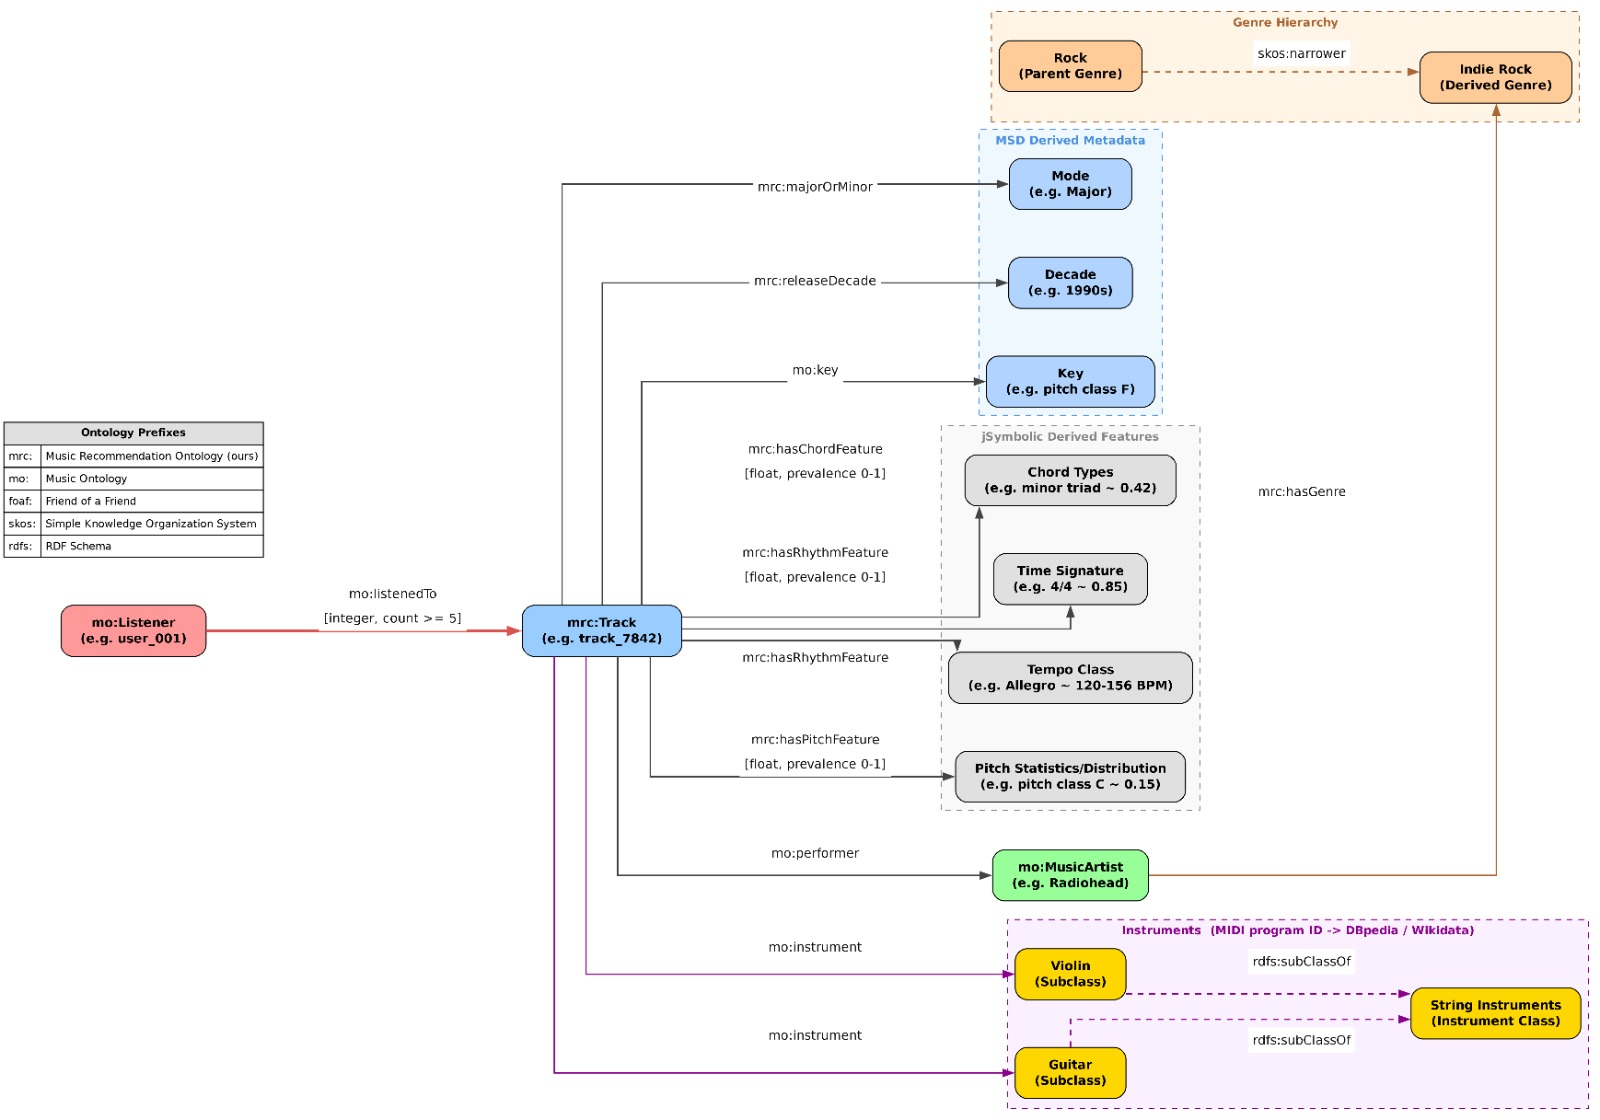
\includegraphics[width=0.75\linewidth]{sec/figures/KG.jpeg}
    \caption{Graphical overview of the proposed methodology.}
    \label{fig:KG}
\end{figure}

The graph will be populated by integrating the filtered user interaction data with the Lakh/MSD dataset and the extracted musical features, using shared identifiers such as song ID and MIDI file mappings. This unified representation will enable the combination of relational, contextual, and musical information, forming the foundation for subsequent graph-based learning and recommendation models.

\subsection{Modeling}

The main model utilized for this project will be a \textbf{Convolutional Graph Neural Network}, a recommendation model that uses the previously constructed knowledge graph to predict which new songs a user is likely to enjoy. It should be noted, however, that the knowledge graph will not be directly used in its raw form, but will require transformation into a graph representation suitable for neural processing, including the incorporation of node attributes and interaction information. This additional modeling step will allow for the integration of both relational structure and numerical feature representations, making the approach more flexible and expressive.

Additionally, a simple \textbf{KNN} or \textbf{Collaborative Filtering Model} will be created to serve as a baseline. This model will rely solely on user interaction data and will be based on standard approaches such as Matrix Factorization and its neural extensions (Neural Collaborative Filtering). It will help us evaluate whether the proposed approach, which integrates the knowledge graph and musical features, performs better and therefore brings value to the recommendation system by improving prediction accuracy and personalization beyond traditional interaction-based methods.

\subsection{Evaluation}

The evaluation process will be conducted using two complementary approaches. First, standard evaluation metrics will be used to assess how well each model performs in predicting user preferences. The dataset will be split into training and test sets at the level of user–song interactions after preprocessing. Only the interaction data will be divided, while all song-related features and metadata will remain available to both sets. The models will be trained using the training interactions, together with the full set of musical features, whereas the test interactions will be used exclusively for evaluation in order to avoid information leakage. Second, the performance of the proposed model will be compared against a baseline collaborative filtering model to determine whether the inclusion of the knowledge graph and musical features leads to improved recommendation quality.

In terms of evaluation metrics, both unoptimized and optimized measures will be considered. Hit Rate will be used as a standard, unoptimized metric, as it provides a straightforward indication of whether relevant items appear in the recommendation list. In addition, a weighted combination of metrics such as Accuracy, Recall, NDCG (Normalized Discounted Cumulative Gain), and Coverage will be used as optimized evaluation criteria. The use of both unoptimized and optimized metrics will allow us for a more comprehensive evaluation, providing us with intuitive baseline understanding of performance, as well as a more nuanced assessment that balances accuracy, ranking quality, and diversity of recommendations.

\subsection{Methodology Pipeline}
\begin{figure}[t]
    \centering
    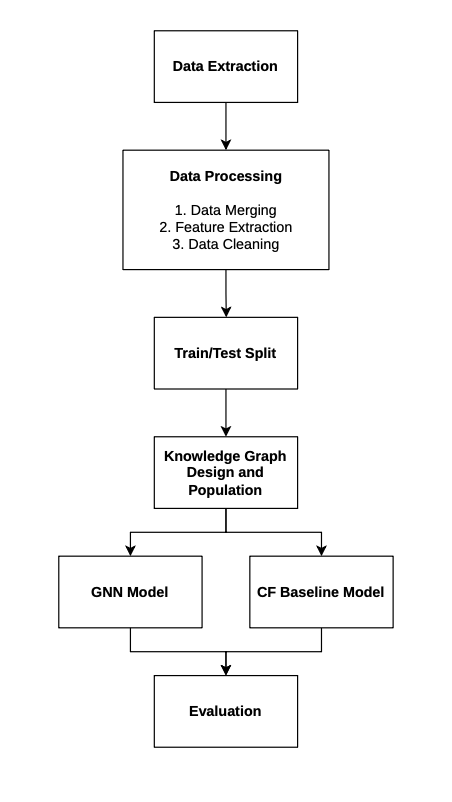
\includegraphics[width=0.75\linewidth]{sec/figures/methodology.png}
    \caption{Graphical overview of the proposed methodology.}
    \label{fig:methodology}
\end{figure}

To better illustrate the overall approach adopted in this project, a visual representation of the methodology is provided in Figure~\ref{fig:methodology}. The figure summarizes the key stages of the proposed pipeline, including data processing, knowledge graph construction, model development, and evaluation. 

This project is currently in the Data Processing and Knowledge Graph Design step, which include feature selection and feature engineering, constituting for a crucial component of the overall design. One of the expected, future key challenges will be determining which musical attributes should be explicitly represented as nodes within the knowledge graph, and which should instead be modeled in a different form, having in mind that it will directly affect both the interpretability and the scalability of the graph. 

The subsequent significant difficulty we expect to encounter will be transforming the knowledge graph into a graph representation suitable for neural processing, where both the relational structure and selected feature information are incorporated. This will have to be performed directly before the modeling step, and will constitute an important part of the methodology, as it determines how effectively the model can leverage both structural and musical information for recommendation tasks.
